\documentclass[10pt,a4paper]{article}
% Styling adapted from the tracked GitHub report progress_reports/2026-10-01.
% Standalone source: all tables and the figure are embedded, no external assets.
\usepackage[margin=1.8cm]{geometry}
\usepackage[T1]{fontenc}
\usepackage[utf8]{inputenc}
\usepackage{lmodern,microtype,booktabs,tabularx,array,amsmath,enumitem,xcolor,hyperref,tikz}
\hypersetup{colorlinks=true,linkcolor=black,citecolor=black,urlcolor=blue,pdftitle={Thesis Progress Update: Global Complementary-Model Routing},pdfauthor={Eren Olmez}}
\setlength{\parindent}{0pt}
\setlength{\parskip}{0.4em}
\renewcommand{\arraystretch}{1.13}
\setlist[itemize]{leftmargin=1.3em,itemsep=0.1em,topsep=0.2em}
\newcommand{\pp}{\,pp}
\newcommand{\code}[1]{\texttt{#1}}
\newcommand{\pagehead}[1]{\section*{#1}}
\begin{document}
\begin{center}
{\Large\bfseries Thesis Progress Update: Global Complementary-Model Routing}\par
{\normalsize Eren Olmez --- M.Sc. Thesis --- 13 October 2026}\par
{\small Results saved through 12 October 2026; update to the previous 1 October report.}
\end{center}
\vspace{-0.6em}
\pagehead{1. Completed deployment work and numerical status}
\textbf{Main change.} The study expanded from one ResNet-18 pruning family to eight architectures and \textbf{213 deployment configurations}. A completed small-data correctness-routing baseline now shows some measured advantages over accuracy-matched static inference, but neither consistent superiority nor the full PC/Jetson study is established. The general motivation and introductory literature survey from the previous report are omitted here.

\begin{tabularx}{\linewidth}{@{}Xrl@{}}
\toprule Stage & Saved progress & Interpretation \\
\midrule
FP32 source models / ONNX export & 71/71 & 8 baselines + 63 pruning variants \\
Diagnostic precision accuracy & 213/213 & Completed; heterogeneous runtimes \\
PC TensorRT static targets & 213/213 & 6,390 timing/energy repetitions \\
Within-architecture scalar controls & 1,941 routes & Stopped; not global progress \\
Global scalar routing & 52/1,440 & Stopped for correctness-method switch \\
213-output correctness baseline & 120/120 & Complete; 53 accuracy-compliant \\
Jetson architecture engines / accuracy & 75/213 & Paused, target-native builds \\
Jetson fully measured static targets & 74/213 & 2,232/6,390 saved repetitions \\
\bottomrule
\end{tabularx}

\textbf{Export and accuracy checks.} All 71 ONNX sources passed 213 PyTorch/ONNX checks at batches 1, 8 and 128; maximum absolute logit error was 0.000280, with matching top-1 predictions on the checked sample (67.31\,s total). Sources occupy 1.70\,GB. Fixed INT8 calibration used 1,024 training images. Each PC TensorRT target has full 5,000-image validation and 10,000-image test predictions; batches 1/8/16/32/64/128 each have five static repetitions. Execution success did not imply accuracy success.

\textbf{Unpruned deployment results.} Test top-1 accuracies below are actual PC TensorRT measurements. FP16 latency is normalized-host-input to logits, \emph{per batch of 32}; energy is GPU mJ/image. These static boundaries are narrower than the routed RGB-to-prediction boundary. Values are arithmetic means of the five saved repeats, not directly comparable with Jetson measurements.

\begin{center}\small
\begin{tabular}{@{}lrrrrrr@{}}
\toprule Architecture & FP32\% & FP16\% & INT8\% & FP16 ms/b32 & mJ/image & Fit min$^{a}$ \\
\midrule
ResNet-18 &79.16&79.17&77.66&9.131&8.830&90.14\\
ResNet-34 &81.82&81.85&73.41&7.451&10.055&156.38\\
ResNet-50 &84.39&84.38&79.69&25.882&25.075&348.67\\
ResNet-101 &85.80&85.85&66.80&42.447&40.749&216.95\\
MobileNetV3-Small &62.38&62.36&15.50&2.709&2.904&24.72\\
MobileNetV3-Large &81.34&81.32&30.77&4.053&5.143&103.31\\
EfficientNet-B0 &82.73&82.71&13.59&6.975&9.231&196.34\\
ShuffleNetV2 x1.0 &75.64&75.66&74.66&7.597&7.637&29.12\\
\bottomrule
\end{tabular}
\end{center}
{\footnotesize $^{a}$ Original classifier baseline training durations, not router training or precision conversion. Classifier checkpoints are retained rather than retrained for each precision.}

\textbf{Findings.} FP16 generally preserves accuracy; the diagnostic, non-uniform-runtime precision study found a mean FP16 loss of 0.08\pp and an INT8 loss of 21.08\pp relative to matched FP32 pruning levels. These are diagnostic accuracy statistics, \emph{not} GPU speedup statistics. EfficientNet-B0's diagnostic p0 INT8 loss was 69.16\pp; its actual TensorRT p0 INT8 accuracy is only 13.59\%. Integer compute was independently inspected: p0 INT8 integer-layer counts are 16/26/54/105 for ResNet-18/34/50/101, 54/64 for MobileNet Small/Large, 82 for EfficientNet and 57 for ShuffleNet. Integer execution does not guarantee useful quantization accuracy.

\newpage
\pagehead{2. Approaches stopped or superseded: what they showed}
\textbf{Pruning and screening.} All sources remain available, but the initial strict-accuracy shortlist was not useful as a global routing pool. At a 2\pp test-accuracy screening allowance, only MobileNetV3-Small p10 joined the eight p0 sources: p0 62.44\%, p10 60.82\%, loss 1.62\pp, MAC reduction 27.11\%. No pruned ResNet, EfficientNet or MobileNet-Large qualified under that screening. The nine-source/27-target shortlist was \emph{superseded}, not used to restrict the eventual 213 choices. Screening used historical test accuracy and is therefore descriptive, not a valid independent selection procedure; runtime policies now select/calibrate on validation data. More aggressive pruning and failed quantization are preserved in the catalogue, not silently discarded.

\textbf{Scalar controls.} Scalar supervision compresses cheapest-correct, cost-ordered candidate behavior into one score. It is not a vector estimating each model's correctness. Direct scalar methods were the gradient stump, batch depth-3 tree, batch logistic, depth-2 XGBoost and batch TinyCNN. Image-tree controls aggregated scalar scores with mean or percentiles 10/25/50/70/80/90. Scalar logistic predicted a binary rank-related target, \emph{not} 213 independent correctness probabilities.

\begin{center}\small
\begin{tabular}{@{}lrrrr@{}}
\toprule Within-architecture control & Saved & Accuracy pass & Positive latency$^{b}$ & Positive energy$^{b}$\\
\midrule
Gradient stump &180&180&48&42\\
Batch tree d3 &161&152&71&64\\
Batch logistic &160&103&2&1\\
Batch XGBoost d2 &160&120&59&53\\
Batch TinyCNN &160&85&1&1\\
Image tree: mean &160&100&49&44\\
Image tree: p10 &160&128&44&42\\
Image tree: p25 &160&122&50&47\\
Image tree: p50 &160&153&68&62\\
Image tree: p70 &160&147&69&61\\
Image tree: p80 &160&151&65&59\\
Image tree: p90 &160&157&68&60\\
\midrule
Total &1,941&1,598&594&536\\
\bottomrule
\end{tabular}
\end{center}
{\footnotesize $^{b}$ Positive savings among accuracy-compliant rows against the recorded eligible static comparator. Rows pool architectures, budgets, objectives and seeds; cached comparators and timing variation make these \emph{control observations}, not confirmed independent wins.}

\textbf{Why stop within-architecture tests?} They could not answer the revised research question: choosing between \emph{all} architectures, precisions and pruning configurations. Their 1,941 measurements were retained as controls, never added to global completion counts. The global scalar protocol instead exposed all 213 logical choices with a capacity-two resident engine cache and fresh static comparators.

\begin{center}\small
\begin{tabular}{@{}lrrrr@{}}
\toprule Global scalar method & Saved & Accuracy pass & Positive latency$^{c}$ & Positive energy$^{c}$\\
\midrule
Gradient stump &20&20&2&2\\
Batch tree d3 &20&20&2&2\\
Batch logistic &12&5&0&0\\
\midrule Total &52&45&4&4\\
\bottomrule
\end{tabular}
\end{center}
{\footnotesize $^{c}$ Same count definition as above; fresh but sequential comparators. XGBoost, TinyCNN and image aggregates had no saved global measured routes at the priority switch. The 52 rows are only 3.61\% of the originally planned 1,440-case global matrix.}

\textbf{Why switch to correctness?} A scalar rank can obscure non-monotonic model strengths: a model with worse total accuracy may rescue specific errors of the best model. Scalar routing was stopped at an atomic completed configuration on user request, not declared fully evaluated or universally inferior. Apparent scalar wins also exposed nonstationarity: one batch-64 policy selected ResNet-101 FP16 for \emph{every} image, while five routed passes were approximately 22.00/22.04/15.21/14.58/14.59\,s and preceding same-model static passes about 21.26/21.24/21.32/21.28/21.34\,s. Such a win cannot be attributed to model selection. A later same-model comparison had 3.21\% \emph{more} routed energy. Timing diagnostics/interleaved confirmation remain necessary.

\newpage
\pagehead{3. Complementarity audit and the 213-output router}
\textbf{Validation-only means no held-out test supervision.} The 5,000 classifier-validation images supplied offline correctness labels; for each seed 42/45/48, 3,000 images fitted the router and 2,000 calibrated its policy. The router therefore \emph{was trained}; this is not a validation-only accuracy check without learning. Calibration did not train weights, and 10,000 held-out test images were opened only for final evaluation. The base classifiers' validation set had already informed their checkpoint selection, which remains a methodological limitation.

\textbf{Audit results.} Validation-selected ResNet-101 p0 FP32 obtained 85.88\%. A label-aware per-image oracle over all 213 candidates obtained 99.28\%: only 36/5,000 images were wrong for every candidate. The eight unpruned FP32 architectures alone gave an oracle accuracy of 95.68\%. These are upper bounds that know the true labels, not deployable results or energy savings. MobileNet-Large p0 FP16 rescued 250 reference errors but introduced 441 errors; EfficientNet p0 FP16 rescued 246 and introduced 383. This explains why unconditional replacement can hurt while conditional selection could help.

\begin{center}
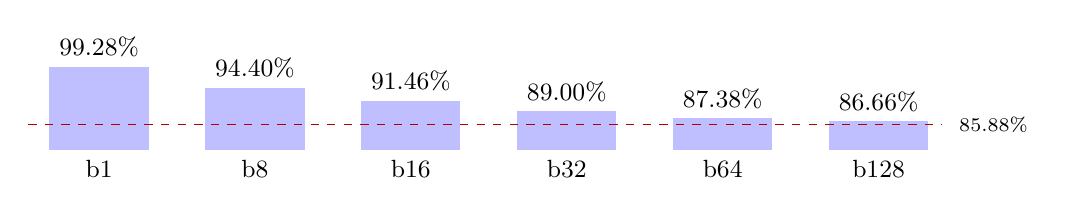
\begin{tikzpicture}[x=0.09cm,y=0.055cm]
\foreach \x/\v/\label in {0/99.28/1,22/94.40/8,44/91.46/16,66/89.00/32,88/87.38/64,110/86.66/128}{
  \fill[blue!25] (\x,0) rectangle +(14,{\v-80});
  \node[font=\small,above] at ({\x+7},{\v-80}) {\v\%};
  \node[font=\small,below] at ({\x+7},0) {b\label};
}
\draw[dashed,red!70!black] (-3,5.88)--(126,5.88);
\node[anchor=west,font=\scriptsize] at (127,5.88) {85.88\%};
\end{tikzpicture}
\end{center}
{\small Ideal one-model-per-batch accuracy for one fixed validation shuffle. Bars start at 80\%; dashed line is the best static validation accuracy. Batching amortizes overhead but removes most of the per-image oracle headroom: b128 gives only 0.78\pp above the reference, versus 13.40\pp for per-image selection.}

\textbf{Implemented model.} A 16$\times$16 input thumbnail feeds a lightweight depthwise encoder with a shared 213-logit head. Independent binary cross-entropy targets indicate whether \emph{each} candidate predicts the true label; multiple heads can be correct. Training used 20 fixed epochs, Adam at 0.001, no test-based checkpoint selection. For a real batch $B$, selection uses
\[
q_m(B)=|B|^{-1}\sum_{x\in B}\sigma(z_m(x)),\qquad
m^*(B)=\arg\max_{m\in\{1,\ldots,213\}}\left[q_m(B)-\lambda\frac{C_m(B)}{\max_j C_j(B)}\right].
\]
The accuracy allowance constrains the \emph{overall calibrated policy}, not each individual model's global accuracy. No candidate shortlist prevents a weaker specialist from being selected. Latency and energy have independent calibration; allowances are 0.5/1/1.5/2\pp. Nominal static costs guide policy calibration; end-to-end measurement is required to learn whether the resulting system actually saves cost.

\textbf{Verified fit/export milestone.} Three shared fits and six objective/seed calibration groups completed. Each seed has six fixed-shape TensorRT router engines including the genuine tail batch of 16. Maximum PyTorch/TensorRT output discrepancy was $2.3842\times10^{-7}$ (seed 48: $1.7881\times10^{-7}$); epoch, weights, source/split and engine provenance were retained. Stage times below include fitting/export/calibration, not classifier training. Lower fitting BCE does not by itself establish generalization or end-to-end savings.
\begin{center}\small
\begin{tabular}{@{}rrrr@{}}
\toprule Seed & Stage seconds & Epoch-1 fitting BCE & Epoch-20 fitting BCE\\
\midrule42&53.72&0.65984&0.45293\\45&46.00&0.63925&0.44929\\48&42.52&0.65903&0.45325\\\bottomrule
\end{tabular}
\end{center}

\textbf{Relationship to prior work.} Correctness-style supervision was already implemented in the earlier 10-candidate router benchmark; the new work expands it to 213 measured deployment choices and a stricter held-out/runtime protocol. PERTINENCE is the closest input-based model-selection neighbor \cite{pertinence}; Taylor et al. also select models before inference on embedded systems \cite{taylor}. Benefit-aware rather than appearance-only difficulty is consistent with DynamicDet \cite{dynamicdet}; CARN and adaptive-inference policies provide related alternatives \cite{carn,adaptive}. The novelty claim must concern the measured joint architecture/precision/pruning system, not the existence of a router or an oracle.

\newpage
\pagehead{4. Complete correctness matrix: all 120 saved tests}
{\small Each cell is \textbf{accuracy loss (pp) / latency saving (\%) / GPU-energy saving (\%)} for one seed. Savings are against that row's frozen validation-eligible, freshly measured static comparator; negative values mean slower/more energy. A superscript $*$ marks a held-out accuracy-budget failure, even if savings are positive. Five full 10,000-image repeats per cell. Results are descriptive, never used to retune the policy.}
\begin{center}
\footnotesize\renewcommand{\arraystretch}{1.14}
\begin{tabular}{@{}lrrlll@{}}
\toprule Objective &Batch&Budget& Seed 42: loss / L / E & Seed 45: loss / L / E & Seed 48: loss / L / E\\
\midrule
Latency&8&0.5&0.26 / -143.7 / -150.8&0.33 / +0.6 / +1.1&1.50 / -20.2 / -22.7$^*$\\
&8&1&0.75 / -513.9 / -430.5&1.51 / -36.5 / -39.1$^*$&1.83 / -19.2 / -21.9$^*$\\
&8&1.5&1.33 / -712.9 / -472.7&1.71 / -55.0 / -58.9$^*$&2.59 / -198.2 / -210.3$^*$\\
&8&2&1.83 / -713.7 / -350.7&2.15 / -94.2 / -101.9$^*$&3.10 / -222.9 / -240.3$^*$\\
&16&0.5&0.28 / -122.9 / -94.1&1.09 / +11.5 / +11.6$^*$&0.28 / -0.6 / -0.7\\
&16&1&0.88 / -191.7 / -129.1&1.52 / +18.4 / +18.5$^*$&0.81 / +6.2 / +5.9\\
&16&1.5&2.00 / -222.4 / -151.0$^*$&1.89 / +23.4 / +23.7$^*$&2.03 / -18.6 / -18.4$^*$\\
&16&2&2.82 / -85.1 / -50.2$^*$&2.40 / +30.6 / +30.5$^*$&2.03 / -18.7 / -19.6$^*$\\
&32&0.5&0.45 / +0.7 / +0.4&0.71 / +4.3 / +4.4$^*$&0.85 / +12.9 / +13.5$^*$\\
&32&1&0.84 / +6.0 / +5.4&0.79 / +7.2 / +6.8&1.42 / +21.6 / +21.2$^*$\\
&32&1.5&1.38 / +16.6 / +16.3&1.05 / +10.3 / +9.8&1.42 / -18.3 / -18.3\\
&32&2&2.30 / +58.5 / +57.9$^*$&1.57 / +18.3 / +17.6&2.31 / -5.8 / -6.3$^*$\\
&64&0.5&0.87 / +13.2 / +13.0$^*$&0.28 / +2.5 / +2.5&0.39 / +4.6 / +4.5\\
&64&1&1.78 / +26.7 / +26.2$^*$&0.63 / +6.8 / +6.9&0.96 / +11.4 / +11.1\\
&64&1.5&1.78 / +26.7 / +26.6$^*$&1.22 / +11.4 / +10.9&0.96 / -45.7 / -44.9\\
&64&2&2.72 / +43.7 / +43.2$^*$&2.57 / +28.3 / +27.1$^*$&3.94 / +45.4 / +45.0$^*$\\
&128&0.5&0.57 / +7.8 / +7.6$^*$&0.87 / +11.8 / +11.5$^*$&0.61 / +9.0 / +8.6$^*$\\
&128&1&1.78 / +32.2 / +32.4$^*$&0.87 / +11.8 / +11.1&0.86 / +16.0 / +15.8\\
&128&1.5&1.78 / +32.1 / +32.5$^*$&1.87 / +27.1 / +26.2$^*$&0.86 / -47.7 / -48.2\\
&128&2&1.78 / +32.0 / +32.6&1.87 / +26.9 / +25.5&3.55 / +24.5 / +24.6$^*$\\
\midrule
Energy&8&0.5&0.28 / -109.5 / -117.8&0.28 / +0.4 / +0.3&0.77 / -118.8 / -125.5$^*$\\
&8&1&0.68 / -332.4 / -329.1&1.47 / -1.6 / -3.5$^*$&1.66 / -286.9 / -290.7$^*$\\
&8&1.5&1.07 / -545.2 / -418.9&1.86 / -6.8 / -9.4$^*$&3.10 / -1053.0 / -959.5$^*$\\
&8&2&1.43 / -952.4 / -573.4&2.30 / -9.6 / -12.5$^*$&3.44 / -1304.0 / -857.2$^*$\\
&16&0.5&0.30 / -180.0 / -150.6&1.10 / +11.8 / +11.6$^*$&0.25 / -4.9 / -2.8\\
&16&1&0.85 / -279.8 / -212.2&1.55 / +18.7 / +18.0$^*$&0.79 / +6.5 / +5.6\\
&16&1.5&1.77 / -392.1 / -277.2$^*$&1.90 / +23.7 / +23.8$^*$&1.96 / -51.2 / -53.9$^*$\\
&16&2&2.78 / -404.9 / -280.8$^*$&2.42 / +30.6 / +29.7$^*$&3.01 / -42.2 / -36.3$^*$\\
&32&0.5&0.67 / -33.1 / -14.5$^*$&0.75 / +4.7 / +4.8$^*$&1.27 / +16.7 / +16.4$^*$\\
&32&1&0.67 / -8.3 / -10.7&0.79 / +7.1 / +7.5&1.27 / +19.1 / +19.1$^*$\\
&32&1.5&1.68 / +1.7 / -0.1$^*$&1.05 / +10.4 / +10.4&1.27 / -21.8 / -28.4\\
&32&2&2.17 / +13.4 / +12.7$^*$&1.61 / +18.5 / +17.9&1.97 / -8.2 / -9.5\\
&64&0.5&0.57 / +8.3 / +8.0$^*$&0.53 / +5.5 / +5.3$^*$&0.16 / +2.0 / +0.0\\
&64&1&1.36 / +19.6 / +19.6$^*$&1.06 / +9.5 / +9.4$^*$&0.62 / +39.1 / +33.5\\
&64&1.5&1.36 / +19.6 / +19.7&1.46 / +15.5 / +15.6&1.14 / -40.1 / -40.4\\
&64&2&2.29 / +13.8 / +13.0$^*$&2.31 / +29.1 / +28.2$^*$&2.15 / -15.4 / -14.9$^*$\\
&128&0.5&0.41 / +6.2 / +5.9&1.29 / +19.2 / +18.7$^*$&0.41 / +5.4 / +5.1\\
&128&1&1.29 / +15.6 / +15.2$^*$&1.29 / +23.9 / +23.2$^*$&0.68 / +14.2 / +14.5\\
&128&1.5&1.29 / +24.9 / +24.6&1.87 / +27.2 / +25.7$^*$&0.68 / -50.3 / -50.2\\
&128&2&2.72 / +45.6 / +45.6$^*$&1.87 / +27.2 / +26.4&3.51 / +17.8 / +18.2$^*$\\
\bottomrule
\end{tabular}
\end{center}
\textbf{Reading the table.} A larger allowance can yield \emph{worse savings} without worse routed accuracy because a cheaper static model becomes eligible. Conversely, large positive savings with $*$ do not satisfy the experiment's objective. A rounded +0.0\% is a tiny recorded positive value, not meaningful evidence of an energy benefit.

\newpage
\pagehead{5. What the completed router tests establish}
\textbf{Aggregate outcome.} The full matrix is $3\times2\times5\times4=120$ configurations, each with five full test passes: 600 routed passes, or 6,000,000 held-out image evaluations before extra energy-window work. Exactly \textbf{53/120 (44.17\%)} met their held-out accuracy allowance. Of those, \textbf{31} had positive latency savings and \textbf{31} positive energy savings against their recorded eligible static comparator. These counts pool seeds/objectives/allowances, are not 31 independent robust discoveries, and do not replace statistical or interleaved confirmation.

\begin{center}\small
\begin{tabular}{@{}rrrrr@{}}
\toprule Batch & Complete & Accuracy pass & Pass + latency saving & Pass + energy saving\\
\midrule
8&24&10&2&2\\16&24&8&2&2\\32&24&13&9&9\\64&24&11&9&9\\128&24&11&9&9\\
\bottomrule
\end{tabular}
\end{center}
\textbf{Promising but non-universal examples at batch 128.} The following are illustrative rows, \emph{not test-selected policies for deployment}. FP16 comparator identities are R101 except row 4 and row 6, which use R50. Latency is wall-time ms/image and energy is GPU mJ/image, means of five full-test repetitions.
\begin{center}\small
\begin{tabular}{@{}llrrrrrr@{}}
\toprule Objective/seed &Budget &Acc.\%&Loss pp&ms/img&mJ/img&L saving\%&E saving\%\\
\midrule
Latency/42&2.0&84.02&1.78&1.035&31.936&32.05&32.56\\
Latency/45&1.0&84.93&0.87&1.344&41.893&11.83&11.10\\
Latency/48&1.0&84.94&0.86&1.279&39.718&16.00&15.77\\
Latency/48&1.5&84.94&0.86&1.277&39.529&-47.66&-48.21\\
Energy/42&1.5&84.51&1.29&1.144&35.517&24.92&24.64\\
Latency/48&2.0&82.25&3.55$^*$&0.653&20.376&24.49&24.61\\
\bottomrule
\end{tabular}
\end{center}
\textbf{Selection is real, but often concentrated.} Latency/42/b128/2\pp selected R101 FP16 for 5,136 images and R34 FP16 for 4,864. Latency/45/b128/1\pp selected R101 FP16 for 7,040 and EfficientNet FP16 for 2,960. Latency/48/b128/1\pp selected R101 FP16 for 7,424 and R34 FP16 for 2,576. All 213 models were available: selection of only two is a learned/calibrated outcome, not a two-model shortlist. These examples needed two classifier loads and zero evictions per cold-cache repeat. Other configurations can incur many more loads/evictions; every row retains those counts.

\textbf{Measured boundary and why testing took longer.} Each pass includes fresh RGB transfer, GPU normalization, thumbnail/router execution, probability extraction/selection, classifier engine verification/loading/eviction, chosen inference and synchronization. Decode/resize and batch pinning are excluded equally from static and routed paths. Resident capacity two bounds GPU memory, not candidate choice. Fresh reference and eligible-static comparators precede \emph{each} configuration, five repeats each (one measured path if their identities coincide). The router training stage took seconds; millions of actual classifier executions plus fresh comparators and cache work dominated elapsed time. Older screening studies used smaller evaluation sets and/or predicted candidate-only costs, not this boundary.

At b128 the GPU decision component in the examples is approximately 1.30--1.34\,ms/batch; this excludes some host/cache dispatch costs already included in total wall time. NVML energy includes idle/display GPU consumption and excludes CPU/rest-of-PC power. Static costs were gathered earlier and may vary with clocks, temperature and host load; sequential comparisons are not interleaved. Very large b8/b16 slowdowns are retained, not clipped or converted into wins.

\textbf{Conclusion.} There are genuine saved \emph{measured positive rows}, including batch 128; the blanket statement ``routing never helps'' is unsupported. The stronger statement ``correctness routing reliably beats the best static alternative'' is also unsupported: 67 budget failures, seed variation and comparator changes remain. No latency setting in this table passes and improves over its comparator for all three seeds. Oracle bounds must not be confused with learned performance.

\newpage
\pagehead{6. Jetson checkpoint, unfinished work and next priorities}
\textbf{New Jetson architecture study: paused, not finished.} TensorRT 8.6.2 engines are built on Jetson, not copied from PC TensorRT 10.13.3.9 engines. EfficientNet-B0 and MobileNet-Large completed 60 precision targets and 1,800 static repeats. MobileNet-Small then progressed to 15 additional engines/full-accuracy evaluations and 14 fully measured targets. At the preserved shutdown checkpoint there are 75 built/accuracy-validated targets (35.21\%), 74 fully measured targets (34.74\%), and 2,232/6,390 static energy repeats (34.93\%). MobileNet-Small p40 INT8 has 12/30 saved repeats; the last saved point is batch 16, repeat 1. Resume only the remaining repetitions. Three architectures' 60 source/prepared graphs were staged with verified hashes; five architectures still need source transfer.

All completed Jetson accuracy stages use 5,000 validation and 10,000 test images; static targets use batches 1/8/16/32/64/128 with five repetitions and tegrastats energy. The last saved target's GPU maximum was 54.375$^{\circ}$C, \emph{not a live post-shutdown reading}. At user-requested shutdown the exact worker/child were stopped, atomic reports preserved and files synchronized; shutdown was requested successfully and SSH subsequently timed out. Physical power-off was not independently instrumented. \textbf{No new all-architecture/global Jetson routing has been executed}. Older single-family Jetson results in the previous report remain historical controls, not progress toward this new matrix. Full remote per-target numerical reports remain on the paused device; this update uses the verified local count/hash checkpoint rather than inventing unavailable Jetson accuracy/cost values.

\textbf{Why the larger-data stage has not started.} The split audit found exactly 45,000 classifier-training indices and 5,000 validation indices; overlap zero, union all 50,000 training images, \textbf{zero unused reserved images}. All eight classifier summaries share the same split identity. Training a router on the 45,000 images would provide more samples, but correctness supervision would be in-sample for the base classifiers, potentially optimistic. The options are (i) clearly labelled exploratory in-sample supervision with separate validation calibration and test-only final evaluation, or (ii) classifier retraining with a larger reserved router split/out-of-fold predictions, which is cleaner but substantially slower. The choice is pending; neither option has started. Validation-only supervision can be data-limited, but using test labels is not a legitimate remedy.

\textbf{Comprehensive router comparison: implementation prepared, GPU tests pending.} Seven additional 213-output families are implemented: shared depth-1/depth-3 correctness trees, independent logistic heads, depth-2 XGBoost (32 trees per candidate), and restored TinyCNN inputs 8/16/32. The current lightweight 16-input CNN remains a separate baseline, not overwritten. Five suite tests and six related correctness/global-pool tests passed (11 total; 15.699\,s). This proves CPU policy/parity/shape behavior only, not GPU export or savings. In particular, 213 XGBoost ensembles may not be lightweight in deployment.

\textbf{Time-bounded next stage.} After the data-protocol choice: seed 42, objectives latency/energy, batches 32/128, allowances 1/2\pp, one full-test repeat with fresh matched comparators and complete cache/router overhead. Seven methods give 56 preliminary configurations; a newly fitted current-CNN baseline adds eight, giving 64. Label single-repeat findings preliminary. Multi-seed/five-repeat confirmation would expand the seven-method matrix to 840 tests, or 960 including the existing 120-case baseline. Frozen training/tuning/calibration and explicit export/parity checks remain mandatory; never tune from the completed held-out matrix.

\textbf{Reproducibility and scope.} Counts above were recomputed from the saved JSON, not stale progress summaries. The companion \code{numerical\_results.json} preserves all saved PC static/precision rows, 1,941 legacy routes, 52 global scalar routes and 120 correctness routes with per-repeat numbers, selection counts, comparator identities and source SHA256 hashes. It is the numerical supplement to this six-page report. Jetson checkpoint hashes are preserved in \code{jetson\_tests/STAGE\_CHECKPOINT.md}. No abandoned approach is treated as complete, no negative savings/accuracy failures are removed, and no experiment was restarted to produce this document. PC thermal stopping uses two consecutive 85$^{\circ}$C checks at 60-second intervals; CPU temperature is unavailable.

\vspace{-0.5em}
\begin{thebibliography}{9}\footnotesize\setlength{\itemsep}{0pt}
\bibitem{pertinence} O. Shende, G. Ananthanarayanan and M. Traiola, ``PERTINENCE: Input-Based Opportunistic Neural Network Dynamic Execution,'' \emph{IEEE Access}, 2026. \href{https://doi.org/10.1109/ACCESS.2026.3707342}{doi:10.1109/ACCESS.2026.3707342}.
\bibitem{taylor} B. Taylor et al., ``Adaptive Deep Learning Model Selection on Embedded Systems,'' \emph{LCTES}, 2018. \href{https://doi.org/10.1145/3211332.3211336}{doi:10.1145/3211332.3211336}.
\bibitem{dynamicdet} Z. Lin et al., ``DynamicDet: A Unified Dynamic Architecture for Object Detection,'' \emph{CVPR}, 2023.
\bibitem{carn} R. Gaire and A. Roohi, ``CARN: Complexity-Aware Routing Network for Efficient and Adaptive Inference,'' \emph{CVPR Workshop}, 2025.
\bibitem{adaptive} T. Bolukbasi et al., ``Adaptive Neural Networks for Efficient Inference,'' \emph{ICML}, PMLR 70, 2017.
\end{thebibliography}
\end{document}
